% ATIVIDADES REALIZADAS------------------------------------------------------------------

\chapter{\imprimirtitulo}
\label{chap:atividadesRealizadas}
O projeto \imprimirtitulo \space foi concebido com o objetivo de controlar as solicitações de veículos e as viagens realizadas, promovendo uma melhor gestão da frota de veículos do TRE-PB bem como possibilitando a realização de auditorias com base nos dados contidos no sistema.
O sistema é hoje um ativo de TI que foi desenvolvido pela SEDES e está descrito no catálogo técnico de sistemas da COSIS conforme \autoref{fig:figura-ativoTI}. 

\begin{figure}[!htb]
    \centering
    \caption{Catálogo técnico de sistemas - Veículos}
    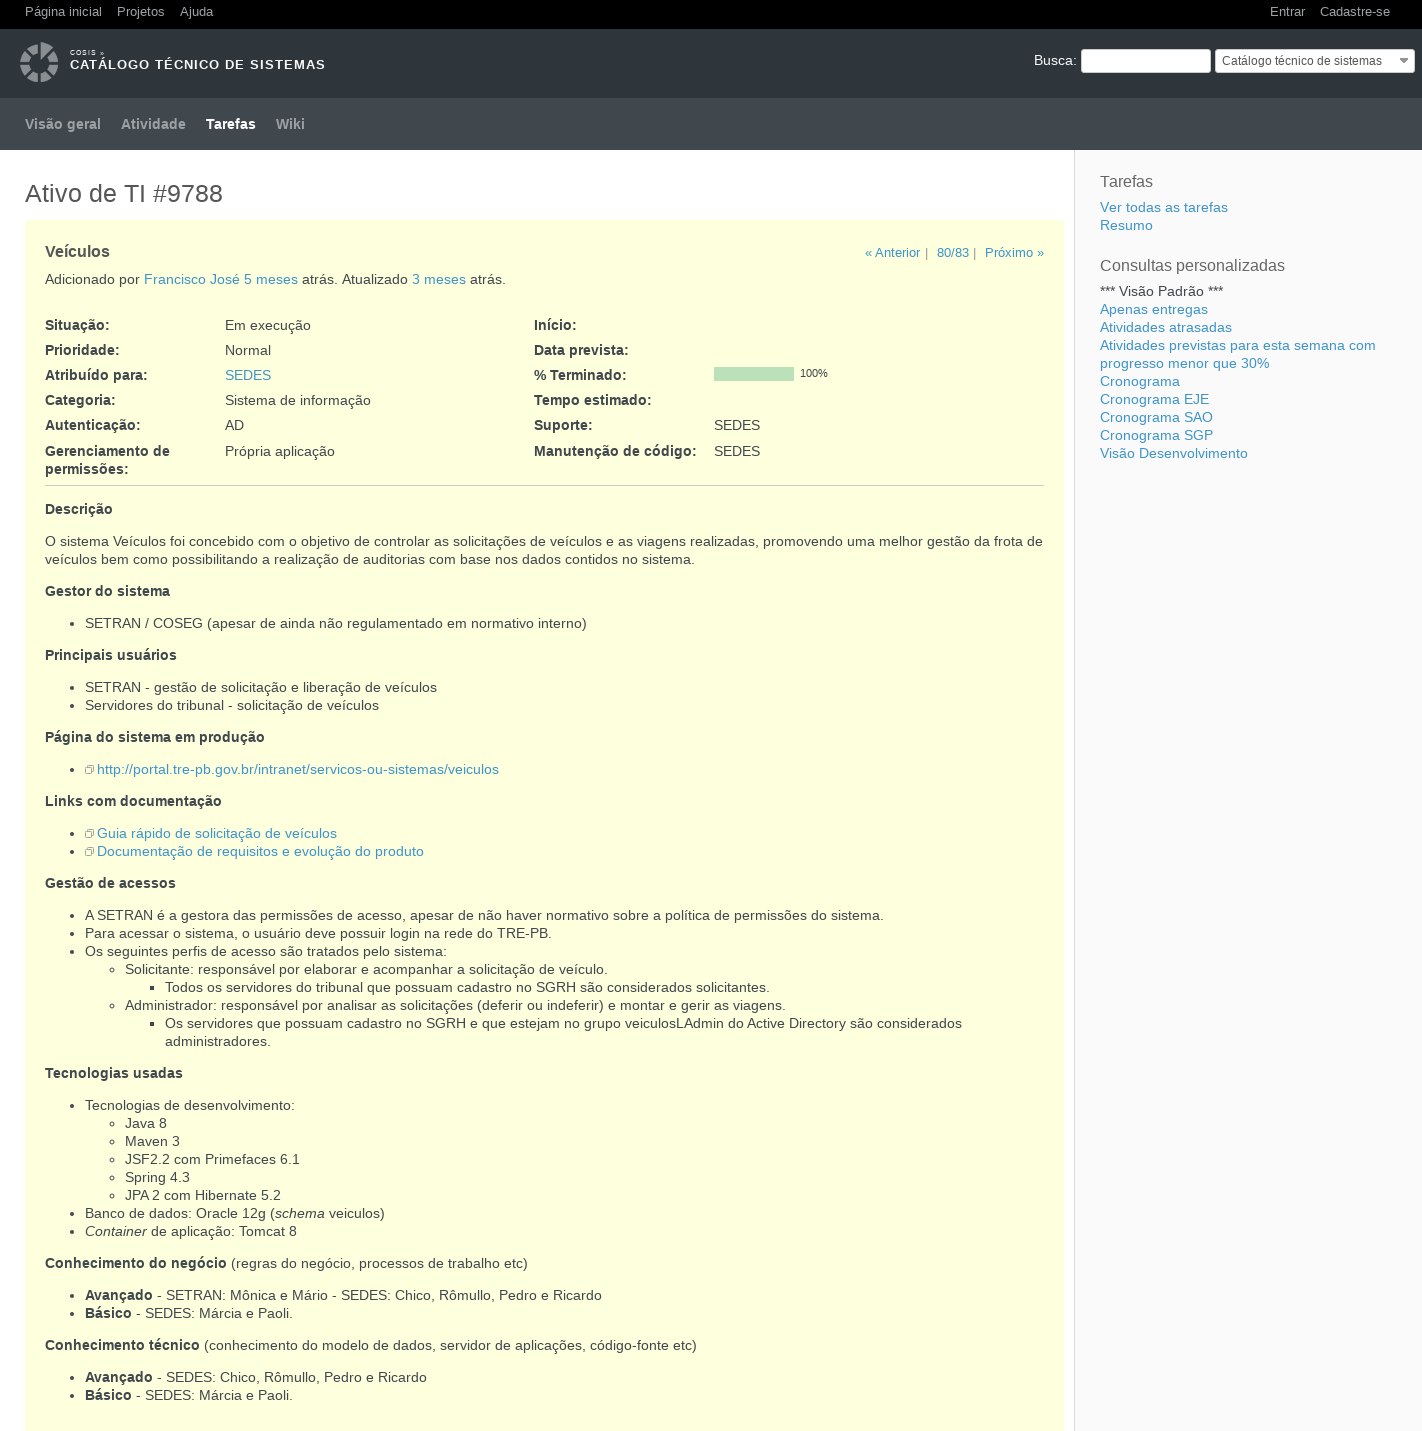
\includegraphics[width=0.75\textwidth]{./dados/figuras/veiculos-ativoTI}
    \fonte{COSIS}
    \label{fig:figura-ativoTI}
\end{figure}

O desenvolvimento do sistema passou por todas as etapas de um projeto de software conforme descrição no modelo de desenvolvimento de software no Anexo \ref{chap:anexoA}. Esse modelo foi construído a partir de definições estabelecidas em portarias, conforme exemplo, no Anexo \ref{chap:anexoB} da última publicada pela Diretoria Geral do TRE-PB no que se diz respeito aos padrões de governança em Tecnologia da Informação.
O processo de desenvolvimento e manutenção de software se inicia com a autorização de análise do problema, visando à elaboração de proposta de solução  \cite[p.~2]{Portaria37:2017}.

Nesse capítulo será explanada minha participação no processo de desenvolvimento do projeto o qual tive a oportunidade de participar desde a concepção, homologação, correção de problemas, criação de uma nova versão com expressiva mudança no modelo de dados e implementação da aplicação em produção. 

\section{A análise do problema}
\label{sec:atividadesRealizadasInicio}

Uma reunião inicial é realizada entre todos os interessados. A COSIS reúne o gestor do sistema, o time de desenvolvimento e o cliente. 

Para o time já se inicia um processo de imersão, onde após ouvir as necessidades descritas pelo cliente começa a imaginar e descrever os possíveis requisitos necessários para a solução. 
Toda reunião realizada entre a equipe e o cliente é descrita cronologicamente e fica publicada na categoria de Atas/Reuniões da SEDES na sitio Wiki do TRE-PB, com a data, hora de início e fim e o nome de todos os participantes, conforme \autoref{fig:figura-ataReuniao1}. Dessa forma todos tem acesso ao que realmente foi solicitado.

\begin{figure}[!htb]
    \centering
    \caption{Ata de Reunião - 21/03/2017}
    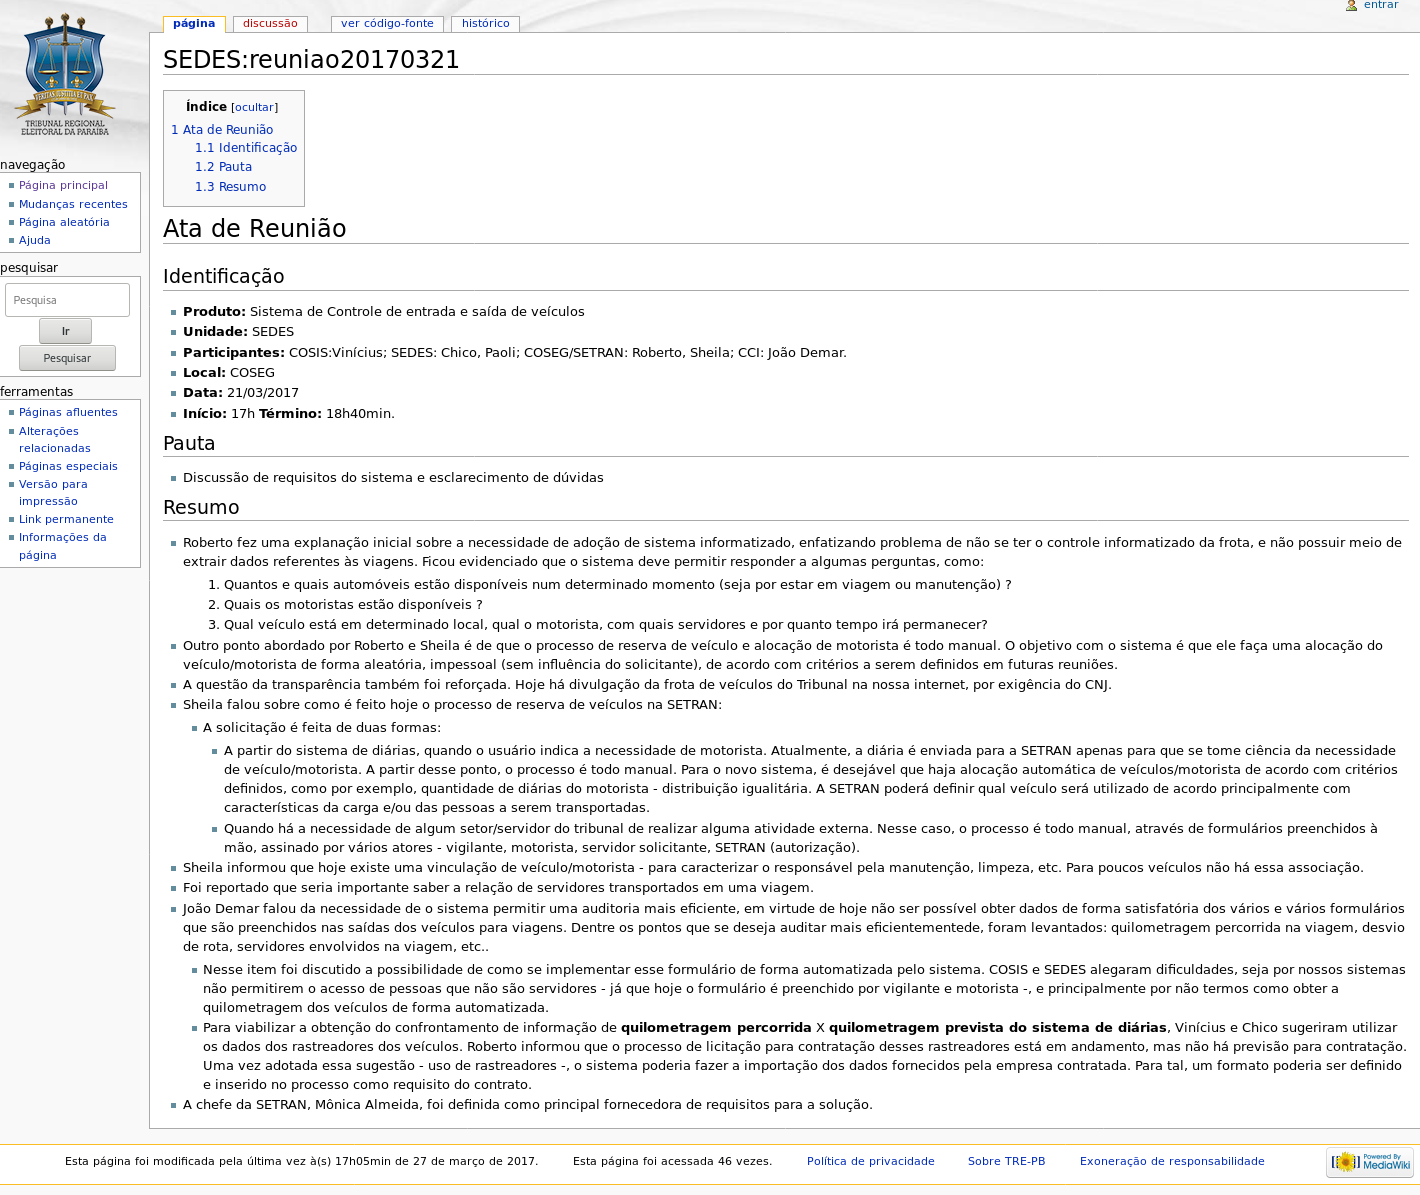
\includegraphics[width=0.9\textwidth]{dados/figuras/veiculos-reuniao20170321}
    \fonte{SEDES}
    \label{fig:figura-ataReuniao1}
\end{figure}

Posteriormente o time volta a se reunir e descrever as histórias de usuário na forma de requisitos a serem implementados. Com os requisitos descritos e cadastrados no sistema de gestão de projetos, o Redmine, na forma de tarefas e atividades, é possível mensurar o tamanho de cada atividade e assim estimar o tempo necessário para conclusão do projeto.  

\section{Planejamento}
\label{sec:atividadesRealizadasPlanejamento}

Todos os membros do time se reúnem para medir o tamanho de cada atividade. Uma a uma é analisada e discutida por cada membro do time onde cada um expõe e justifica o tamanho dado através da técnica do Planning Poker. Após um concesso entre todos fica definido o tamanho da atividade. Assim o gerente com esses dados em mãos formaliza o projeto como uma demanda de serviço, contendo o prazo o time necessário para concluir as releases.

\begin{citacao}
Após a autorização, o gestor do sistema promoverá a reunião de
partida entre o time de desenvolvimento e as partes interessadas, momento em que será
esclarecido o problema de negócio, definidos papéis, explicado o processo de
desenvolvimento e distribuídas responsabilidades.\cite[p.~2]{Portaria37:2017}
\end{citacao}

As releases definidas são apresentadas como as versões que serão entregues e são separadas conforme ordem de prioridade das atividades e requisitos como mostra a \autoref{fig:figura-planejamento}.


\begin{figure}[!htb]
    \centering
    \caption{Planejamento das versões}
    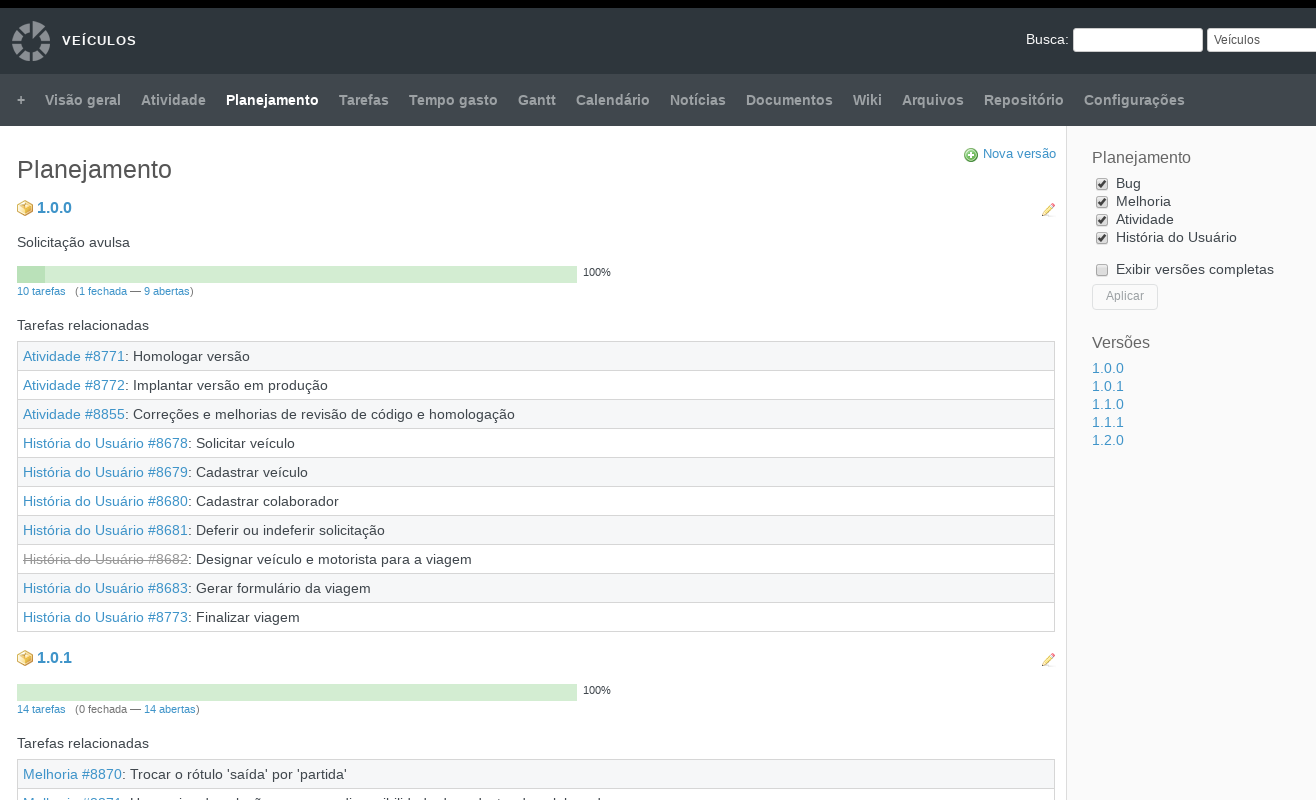
\includegraphics[width=0.75\textwidth]{dados/figuras/veiculos-planejamento.png}
    \fonte{SEDES}
    \label{fig:figura-planejamento}
\end{figure}

\section{Desenvolvimento}
\label{sec:atividadesRealizadasDesenvolvimento}

No início da fase de desenvolvimento são gerados os primeiros artefatos em código que serão comuns para todos os membros do time. O TRE-PB utiliza para controle de versões de seus códigos o sistema de versionamento denominado Subversion (SVN). Um novo repositório é criado para o projeto e um novo projeto com um arcabouço contendo as bibliotecas padrões e um template para as páginas já utilizadas pela SEDES é criado disponibilizado no repositório para todos os desenvolvedores. A SISBAN através de um chamado gera um novo schema no banco de dados Oracle 12g e fornece acesso a todos os desenvolvedores.

Todo esse processo é inicialmente implementado pelo supervisor técnico que geralmente é o desenvolvedor responsável pelo projeto e com mais habilidades e experiência do time.

Nesse momento todas as histórias já estão descritas com uma riqueza maior de detalhes, então são criados tickets e colados em um taskboard na forma de um quadro Kanban visível para todos. Esse quadro contém todas as atividades necessárias que atendem ao escopo do projeto para a release em questão. 

Diariamente são realizadas pequenas reuniões denominadas "daily" entre o gestor do projeto e membros do time com o intuito de detalhar o andamento das atividades, conduzir novas atividades para o time bem como relatar as dificuldades encontradas.

Na \autoref{fig:figura-atividade8940} a seguir é possível ver uma tarefa especifica que foi atribuída a mim. A tarefa cadastrada no Redmine possui uma ligação com o repositório SVN, assim é possível ver e analisar trechos de códigos que foram implementados em cada "commit"\footnote{No contexto de ciência da computação e gerenciamento de dados, commit refere-se à ideia de fazer permanentes um conjunto de mudanças experimentais. Uma utilização popular está no fim de uma transação. Um commit é o ato de enviar. https://pt.wikipedia.org/wiki/Commit}.

\begin{figure}[!htb]
    \centering
    \caption{Atividade 8940}
    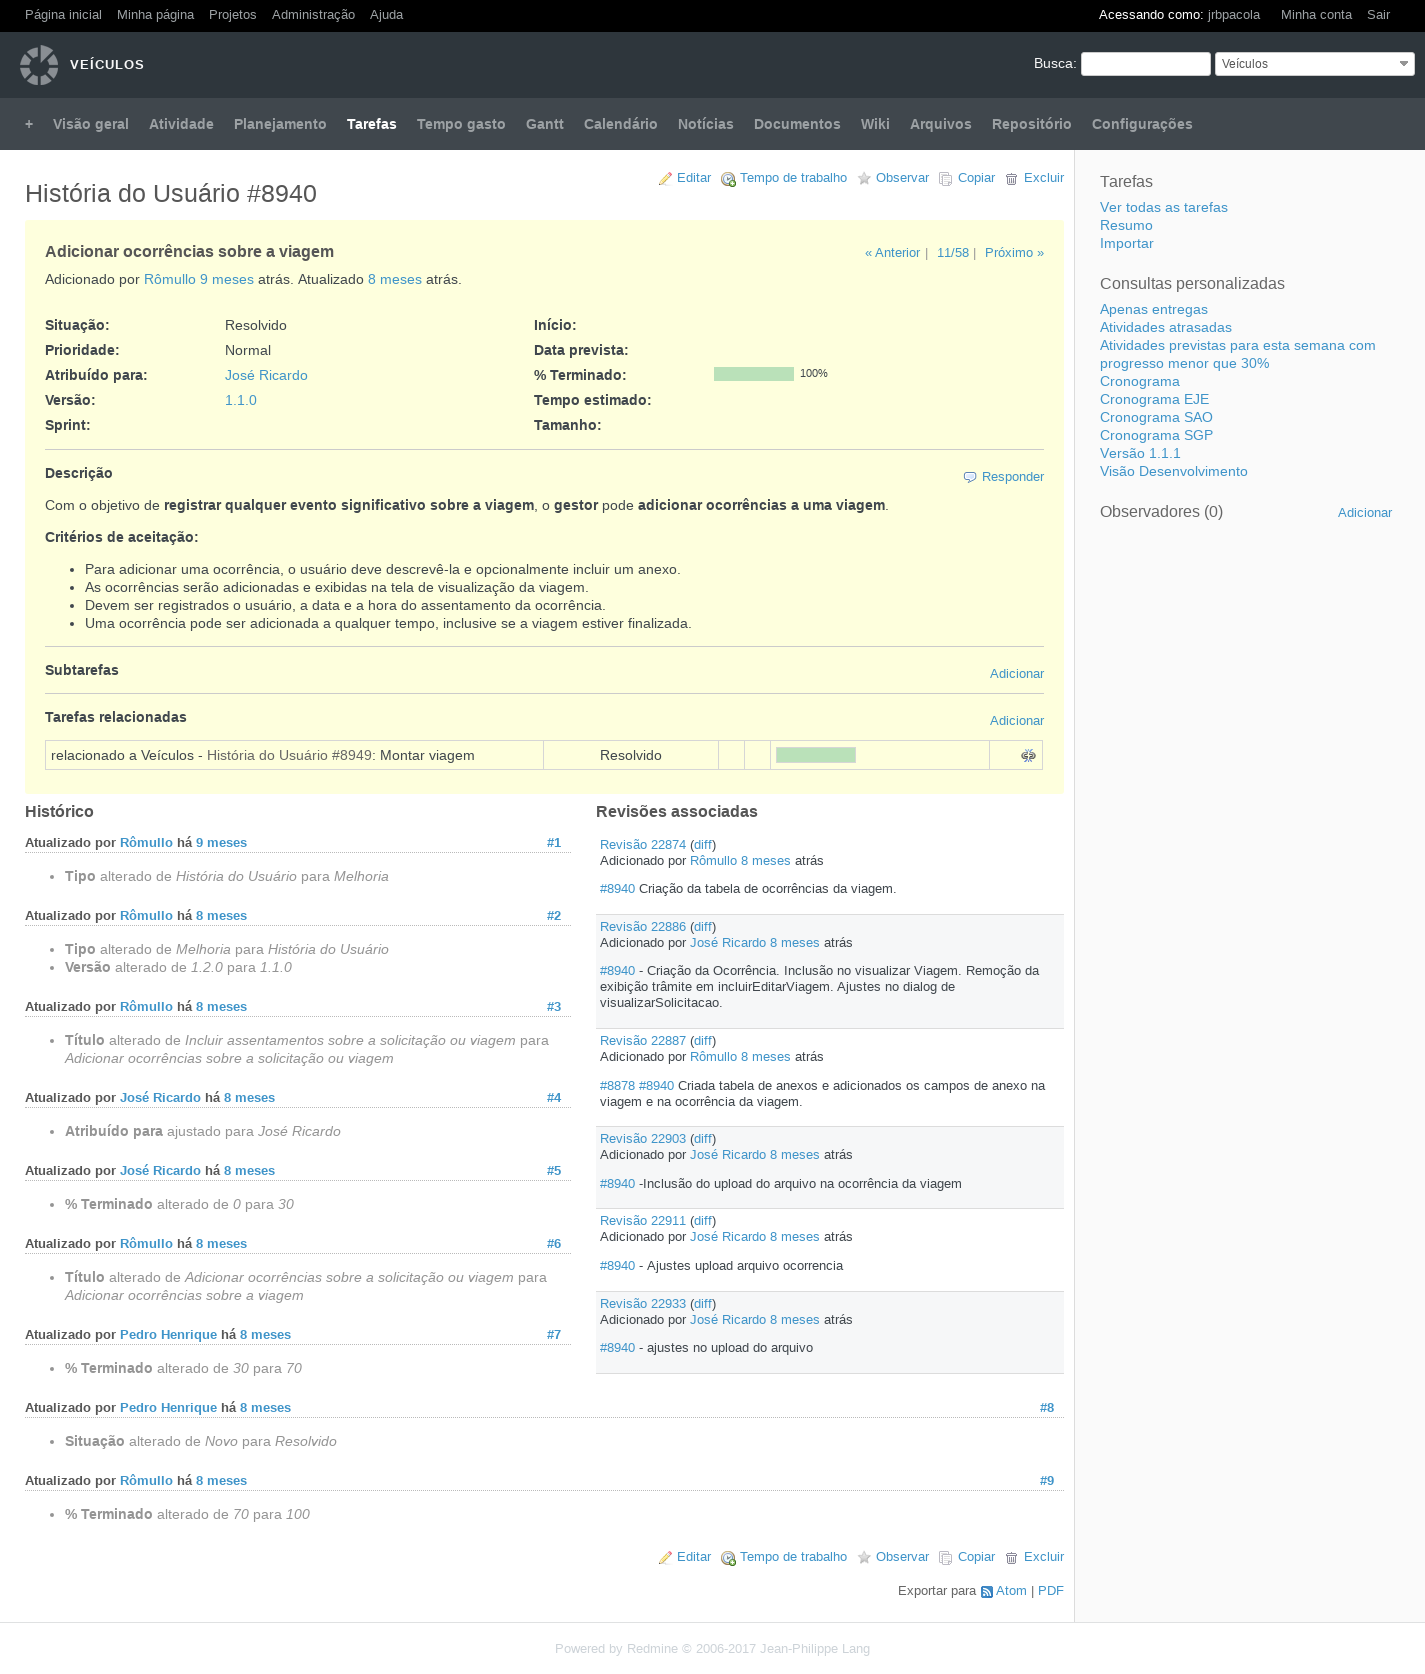
\includegraphics[width=0.75\textwidth]{dados/figuras/veiculos-atividade1.png}
    \fonte{SEDES}
    \label{fig:figura-atividade8940}
\end{figure}

